\documentclass{article}

\usepackage[utf8]{inputenc}
\usepackage{hyperref}
\usepackage{amsmath}
\usepackage{amssymb}
\usepackage{amsthm}
\usepackage{isabelle}
\usepackage{isabellesym}
\usepackage{algpseudocode}
\usepackage{tikz}
\usepackage{stmaryrd}
\usepackage{ifthen}

\newcommand{\iassert}[1]{\mathtt{Assert}(#1)}
\newcommand{\icheck}{\mathtt{Check}()}
\newcommand{\icheckpoint}{\mathtt{Checkpoint}()}
\newcommand{\ibacktrack}[1]{\mathtt{Backtrack}(#1)}
\newcommand{\csat}{\mathtt{Satisfiable}}
\newcommand{\cunsat}{\texttt{Unsatisfiable}}
\newcommand{\cone}{\mathrm{cone}}
\newcommand{\hull}{\mathrm{hull}}
\newcommand{\ints}{\mathbb{Z}}
\newcommand{\ifff}{if and only if}

% Source: https://isabelle.in.tum.de/community/Generate_TeX_Snippets
\newcommand{\DefineSnippet}[2]{%
  \expandafter\newcommand\csname snippet--#1\endcsname{%
    \begin{quote}
    \begin{isabelle}
    #2
    \end{isabelle}
    \end{quote}}}
\newcommand{\Snippet}[1]{%
  \ifcsname snippet--#1\endcsname{\csname snippet--#1\endcsname}%
  \else+++++++ERROR: Snippet ``#1 not defined+++++++ \fi}

\input{../test-cantor-theorem/generated/snippets}
\input{../linear-inequalities-in-isabelle/generated/snippets}

\newtheorem{definition}{Definition}
\newtheorem{theorem}{Theorem}
\newtheorem{corollary}{Corollary}

\title{Internship Report -- Extending a Verified SMT Solver for Mixed-Integer
Linear Arithmetic}
\author{Alban Reynaud}
\date{}

\begin{document}

\maketitle

This work has been done in an internship in the Department of Computer Science
of the University of Innsbruck, under the supervision of René Thiemann, in the
Computer Logic team.

\begin{abstract}
\end{abstract}

\section{Introduction}
\subsection{The Isabelle Proof Assistant}
Isabelle \cite{Isabelle} is a generic proof assistant. Isabelle/HOL
(abbreviation of \textit{Higer Order Logic}) is a specialization that is
generally used.

One of the feature of Isabelle is the use of mathematical symbols to make the
proofs more readable. It also uses automatic provers.
Moreover, there is the language \textit{Isar} that can is used to conduct proofs
in a structured way.

For example, here is a proof of the Cantor Theorem (the fact that there is no
surjection from a set $A$ to its powerset), taken from
\cite[Section 5.1]{ConcreteSemantics}
with Isabelle and Isar:
\Snippet{cantor}

The outline of the proof is the following:
\begin{itemize}
  \item We assume that there exist a surjective function $f$ from $A$ to
    its powerset.
  \item We deduce that there exists an element $a$ of $A$ such that
    $f(a) = \{x~|~x \notin f(x)\}$
  \item But from the following fact we can deduce that both $a \in f(a)$ and $a
    \notin f(a)$ which is a contradiction (represented by the proposition
    $\mathtt{False}$).
\end{itemize}
To prove each of these facts, the automatic provers $\mathtt{blast}$ and
$\mathtt{auto}$ are used.

It is also possible to define objects in the functional programming way in
Isabelle/HOL and to export code. This way, it is possible to have a certified
implementation of an algorithm by writing it in Isabelle/HOL, proving its
correctness and exporting its code.

\subsection{SMT Solving and Linear Arithmetic}
\label{smt}
Let $T$ be a quantifier-free theory. A $T$-solver is an algorithm to check if a
finite set of atom of $T$ can be satisfied.

For example, the theory of \textit{linear arithmetic} is composed of atoms (also
called \textit{constraints}) of the form
$$\sum_{i < n} a_i x_i \bowtie b$$
where $a_0, ..., a_{n-1}, b$ are rational constants, $x_0, ..., x_{n-1}$ are
variables and $\bowtie \in \{=,\leqslant,\geqslant,<,>\}$ is a comparison
operator. An assignement $v$ is a function that maps variables to rationals.
If $c = \sum a_i x_i \bowtie b$ is a constraint,  we say that the assignement
$v$ satisfies the constraint c (or $v \vDash c$) if
$$\sum a_i v(x_i) \bowtie b$$.

Note that we are only interested in the decision problem (\textit{i.e} checking
if a set of constraints admits a satisfying assignment), not the optimization
problem (\textit{i.e} finding an assignment satisfying the constraints that
maximizes a linear objective function). 

The other theory we will study is the theory of \textit{mixed-integer linear
arithmetic}. A mixed-integer linear problem (MILP)
consists of linear problem where some variables are
required to be integer. Furthermore, if all the variables are required to be
integer, the problem is called an \textit{integer linear problem} (ILP).

For example:
\begin{displaymath}
  \left\{
  \begin{array}{cc}
    x + y & \geqslant 3 \\
    y - x & < 2 \\
    x \in \ints
  \end{array}
  \right.
\end{displaymath}
is a MILP.

More formally, if $S$ in a set of linear constraints and $I$ the set of
variables that are required to be integer, if $v$ is a valuation, I will use the
notation $$v \vDash_I S$$ for $v \vDash S$ and
$\forall x_i \in I.~v(x_i) \in \ints$.

Let $\Phi$ be a boolean formula of atoms of the theory $T$. We may want to find
an assignement $v$ that satisfies $\Phi$, or to know if no such assignement
exists. This problem is called \textbf{Satisfiability Modulo Theory} (SMT).

For example, a SMT instance based on linear arithmetic would be:
$$\Phi \equiv (A \vee B \vee C) \wedge (\neg A \vee B) \wedge
              (\neg A \vee C \vee D) \wedge (\neg C \vee D)$$
with
\begin{displaymath}
\begin{array}{lclccc}
  A & \equiv &x  & + & y & \geqslant 3 \\
  B & \equiv &x  &   &   & \leqslant 1 \\
  C & \equiv &   &   & y & \leqslant 1 \\
  D & \equiv &y  & - & x & < 2         \\
\end{array}
\end{displaymath}

Now that SMT and linear arithmetic have been presented, we can move on to the
basics of their resolution.

\subsection{Incremental Interface for SMT solvers}
%TODO: give a chapter number for the book
An efficient procedure to solve SMT problems is DPLL($T$) \cite{Decision2016},
which works as a combination of a SAT-solver and a $T$-solver. Here is a quick
description of such an algorithm:
\begin{itemize}
  \item Replace every atom by a SAT variable to obtain a SAT formula $\Phi$.
    Run a SAT-solver to find a valuation of each variable to 0 or 1 that
    satisfies this SAT-formula.
  \item From this affectation, derive a conjuction of $T$-atoms. Run a
    $T$-solver to find an assignement that satisfies this conjuction.
  \item If an assignment $v$ is found, return $v$
  \item If no assignment is found, from thus conjuction find a contradicting
    subset of atoms. From this subset, derive a new constraint, add it to the
    SAT-formula $\Phi$, and go to the first step.
\end{itemize}

To work efficiently in combination with the SAT-solver, we may assume that the
$T$-solver implements the following interface:
\begin{itemize}
  \item $\iassert{\alpha}$: Asserts the atom $\alpha$. It is added to the set of
    $T$-atoms the should be satisfied.
  \item $\icheck$: Runs a $T$-solver to find an assignment to the set of
    asserted atoms. If such an assignement is found, returns it. Otherwise,
    returns a subset of inconsistent assert atoms.
  \item $\icheckpoint$: Returns a checkpoint $c$ that contains all the necessary
    information to backtrack to the current state.
  \item $\ibacktrack{c}$: Backtracks to the state represented by the checkpoint
    $c$.
\end{itemize}

%TODO: explain why it is called an incremental interface
We will call such an inteface an \textit{incremental interface}.
A similar description can be found in \cite{Dutertre2006} and
\cite{Thiemann2018}.

An example of an execution of DPLL($T$) is given in appendix \ref{dpll}.

Dutertre and de Moura have proposed a Simplex-based solver to solve linear
arithmetic \cite{Dutertre2006}. A partial version of this algorithm has been
formalized in Isabelle by Spasić and Marić \cite{Spasic2012} and extended to
use the incremental interface by Ralph Bottesch, Max Haslbeck and René Thiemann
\cite{Thiemann2018}. The ultimate goal of this internship is to extend the
previous work to solve MILPs.

\section{Resolution of Mixed-Integer Linear Problems}
In this section, I will describe an algorithm to solve MILPs and the mathematics
required to prove its correctness.

\subsection{The Branch-and-Bound algorithm}
\label{bbdescr}
% TODO: give a reference?
Branch-and-bound is a simple algorithm to solve ILPs and MILPs. Though it can be
stated as an optimization algorithm, we will focus on its formulation for
decision problems.

Let $S$ and $I$ be respectively the set of linear constraints and the set of
integral variables of our problem. The principle of the algorithm is the
following:
\begin{itemize}
  \item Search a valuation $v$ such that $v \vDash S$. If no solution exists,
    return \cunsat{}.
  \item If for all $x_i \in I$, $v(i) \in \ints$, then $v \vDash_I S$.
    Return $v$.
  \item If there exists a variable $x_i \in I$ such that
    $v(x_i) \notin \ints$, we can remark that for all solution of this
    MILP, either the constraint $x_i \leqslant \lfloor v(x_i) \rfloor$ 
    or the constraint $x_i \geqslant \lceil v(x_i) \rceil$ is satisfied.
    
    We can then try to split our initial problem into two subproblems (this is
    the \textit{branching step}):
    \begin{itemize}
      \item Recursively call branch-and-bound on the constraints set
        $$S \cup \{x_i \leqslant \lfloor v(x_i) \rfloor\}$$ and $I$.
        If a solution $v'$ is found, return it.
      \item Recursively call branch-and-bound on the constraints set
        $$S \cup \{x_i \geqslant \lceil v(x_i) \rceil\}$$ and $I$.
        If a solution $v'$ is found, return it.
    \end{itemize}
  \item If after the branching step no solution is found, return \cunsat{}.
\end{itemize}

%\begin{algorithmic}[1]
%  \Procedure{Branch-and-Bound}{$S, I$}
%
%  Search for a solution $v$ of $S$
%  \If{no solution $v$ exists}
%    \Return \cunsat{}
%  \ElsIf {$\forall x_i \in I.~v(x_i) \in \ints$}
%    \Return $v$
%  \Else
%    \Return $3v + 4$
%  \EndIf
%  \EndProcedure
%\end{algorithmic}

The problem with this formulation is that the algorithm may loop. For example,
let us examine the following ILP:
\begin{equation} \label{pbloop}
  \left\{
  \begin{array}{l}
    3x - 3y \geqslant 1 \\
    3x - 3y \leqslant 2 \\
    x, y \in \ints \\
  \end{array}
  \right.
\end{equation}

This problem has no solution, and its relaxation (that is the problem composed
by the linear inequalities, without the integrality constaints) is unbounded, as
shown in figure \ref{bbloop}. Here is a possible execution of the
branch-and-bound algorithm on this problem:
\begin{itemize}
  \item Obtain the solution $(\frac{1}{3}, 0)$. The variable $x$ is not
    integral. Try to solve the problem with the extra constaint
    $x \geqslant 1$.
  \item Obtain the solution $(1, \frac{1}{3})$. The variable $y$ is not
    integral. Try to solve the new problem with the extra constraint $y
    \geqslant 1$.
  \item Obtain the solution $(1 + \frac{1}{3}, 1)$. The variable $x$ is not
    integral. Try to solve the problem with the extra constaint
    $x \geqslant 2$.
  \item Obtain the solution $(2, 1 + \frac{1}{3})$. The variable $y$ is not
    integral. Try to solve the new problem with the extra constraint $y
    \geqslant 2$.
  \item etc...
\end{itemize}


\begin{figure}[h]
  \centering

  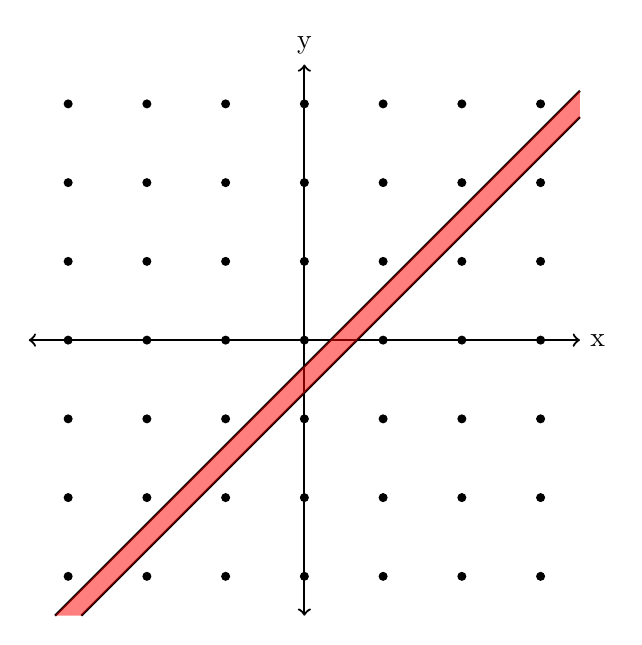
\begin{tikzpicture}
    %\draw[style=help lines,very thin] (-4, -4) grid (4, 4);
    \foreach \x in {-3, -2, ..., 3} {
      \foreach \y in {-3, -2, ..., 3} {
        \node[draw, circle, fill=black, inner sep=1pt] at (\x, \y) {};
      }
    }

    \draw[thick, ->] (0, 0) -- (3.5, 0) node[anchor=west] {x};
    \draw[thick, ->] (0, 0) -- (0, 3.5) node[anchor=south] {y};
    \draw[thick, ->] (0, 0) -- (-3.5, 0);
    \draw[thick, ->] (0, 0) -- (0, -3.5);


    \coordinate (C1LEFT) at (-3.167, -3.5);
    \coordinate (C1RIGHT) at (3.5, 3.167);
    \coordinate (C2LEFT) at (-2.833, -3.5);
    \coordinate (C2RIGHT) at (3.5, 2.833);
    \draw[thick] (C1LEFT) -- (C1RIGHT);
    \draw[thick] (C2LEFT) -- (C2RIGHT);
    \fill[fill=red, opacity=0.5]
      (C1LEFT) -- (C1RIGHT) -- (C2RIGHT) -- (C2LEFT) -- cycle;
  \end{tikzpicture}

  \label{bbloop}
  \caption{Graphical representation of the solutions of the problem
           \ref{pbloop}. The solutions of the relaxation lie in the red area.}
\end{figure}

In this case, the problem is unbounded and makes the branch-and-bound algorithm
loop. This is why we will try to add constraints of the form $-B \leqslant x_i
\leqslant B$ for all variable $x_i$ to bound the problem, at the condition that
the bounded problem admits a solution if and only if the original problem admits
a solution. This is what we are going to see in the next section.

\subsection{Obtening bounds for ILPs and MILPs}
\label{schrijverbnd}
First of all, let us remark that if a linear problem contains only large
inequalities, it could be put in the form:

\begin{displaymath}
  \left\{
  \begin{array}{cccccl}
    a_{11} x_1 & + & ...    & + & a_{1n} x_n & \leqslant b_1 \\
               &   & \vdots &   &            &               \\
    a_{p1} x_0 & + & ...    & + & a_{pn} x_n & \leqslant b_p \\
  \end{array}
  \right.
\end{displaymath}

or in the matrix form $Ax \leqslant b$ with
$$A = (a_{ij})_{\substack{1 \leqslant i \leqslant n \\
                          1 \leqslant j \leqslant p}}$$ and
$b = (b_j)_{1 \leqslant j \leqslant p}$. We identify a valuation of $n$
variables to a vector of dimension $n$.

Now, we are going to give the outline of a proof that MILPs admits a solution
if and only if they admit a solution of small size. In what follows, we will
focus on ILPs, but the results can be easily extended to MILPs. Most of the
definitions and results can be found in Schrijver's book
\cite[Sections 7 and 16]{Schrijver1998}.

\begin{definition}[Finitely Generated Cone]
  A set of points $C$ is a \textup{finitely generated cone}
  \ifff{} $C = \cone~\{x_0, ..., x_{n-1}\}$ where
  $$\cone~\{x_0, ..., x_{n-1}\} =
      \left\{\sum_{i=0}^{i<n} \lambda_i x_i~|~
               \lambda_0, ..., \lambda_{n-1} \geqslant 0\right\}
  $$
  for some $x_0, ..., x_{n-1}$.
\end{definition}

\begin{definition}[Polyhedral Cone]
  A set of points $C$ is a \textup{polyhedral cone}
  \ifff{} $C = \{x~|~Ax \leqslant 0\}$ for some matrix $A$.
\end{definition}

\begin{theorem}[Farkas-Minkowsky-Weyl Theorem]
  A set $C$ is a finitely generated cone \ifff{} it is a polyhedral cone.
\end{theorem}

\begin{definition}[Polyhedron]
  A set of points $P$ is a \textup{convex polyhedron} \ifff{}
  $$P = \{x~|~Ax \leqslant b\}$$
  for some matrix A and vector b.
\end{definition}

Note that a polyhedron could be interpreted as the set of solutions of a linear
problem with only large inequalities.

\begin{definition}[Polytope]
  A set of points $P$ is a \textup{polytope} \ifff{} it is the convex hull of a
  finite set $C = \{x_0, ..., x_{m-1}\}$, \textit{i.e}
  $$P = \left\{
    \sum_{i=0}^{i<m} \lambda_i x_i~|~\lambda_0, ..., \lambda_{m-1} \geqslant 0
                                  \wedge \sum_{i=0}^{i<m} \lambda_i = 1
        \right\}$$
\end{definition}

\begin{corollary}[Decomposition Theorem for Polyhedra]
  A set of points $P$ is a polyhedron \ifff{} there exists a polytope $Q$ and a
  finitely generated cone $C$ such that $P = Q + C$.
\end{corollary}

To illustrate this theorem, let us take the following problem:
\begin{equation} \label{eqdecomp}
  \left\{
  \begin{array}{ccccc}
    -6x & + & 2y & \leqslant & 1  \\
    3x  & + & 2y & \geqslant & 11 \\
        &   & 2y & \geqslant & 1  \\
    2x  & - & 4y & \leqslant & 5
  \end{array}
  \right.
\end{equation}

As we have seen, the set of the solutions of this problem is a polyhedron. On
the figure \ref{figdecomp}, the polyhedron is represented by the red and blue
areas. As we can see, it is the sum of a polytope (the red triangle) and a cone
($\cone~\{u, v\}$).

\begin{figure}[h]
  \label{figdecomp}
  \centering

  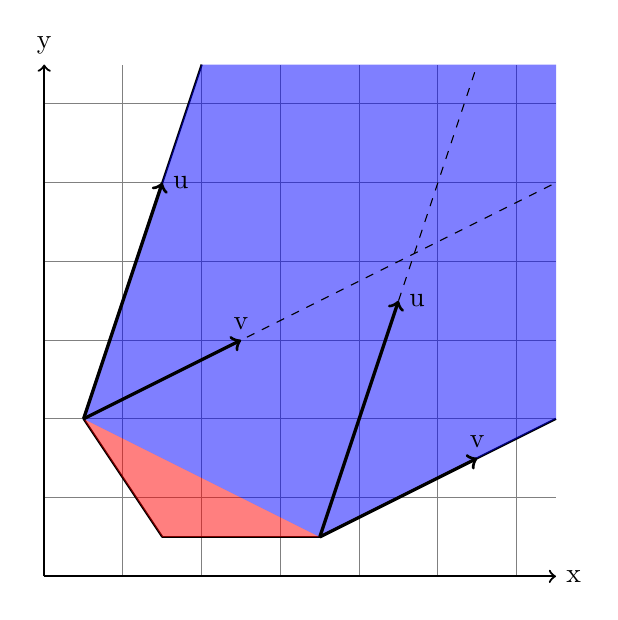
\begin{tikzpicture}
    \coordinate (extr) at (6.5, 6.5);
    \draw[style=help lines, thin] (0, 0) grid (extr);
    \draw[thick, ->] (0, 0) -- (6.5, 0) node[anchor=west] {x};
    \draw[thick, ->] (0, 0) -- (0, 6.5) node[anchor=south] {y};

    \coordinate (A) at (2, 6.5);
    \coordinate (B) at (0.5, 2);
    \coordinate (C) at (1.5, 0.5);
    \coordinate (D) at (3.5, 0.5);
    \coordinate (E) at (6.5, 2);
    \coordinate (B') at (6.5, 5);
    \coordinate (D') at (5.5, 6.5);
    \draw[thick] (A) -- (B);
    \draw[thick] (B) -- (C);
    \draw[thick] (C) -- (D);
    \draw[thick] (D) -- (E);
    \fill[fill=red, opacity=0.5] (B) -- (C) -- (D) -- cycle;
    \fill[fill=blue, opacity=0.5] (A) -- (B) -- (D) -- (E) -- (extr) --
                                  cycle;

    \draw[very thick, ->] (B) -- (1.5, 5) node[anchor=west] {u};
    \draw[very thick, ->] (B) -- (2.5, 3) node[anchor=south] {v};
    \draw[very thick, ->] (D) -- (4.5, 3.5) node[anchor=west] {u};
    \draw[very thick, ->] (D) -- (5.5, 1.5) node[anchor=south] {v};
    \draw[dashed] (B) -- (B');
    \draw[dashed] (D) -- (D');
  \end{tikzpicture}

  \caption{Decomposition of the polyhedron defined by the problem
           \ref{eqdecomp}}
\end{figure}

\begin{corollary}
  $P$ is a polytope \ifff{} $P$ is a bounded polyhedron.
\end{corollary}

\begin{definition}[Integer Hull]
  Given a polyhedron $P$, the \textup{integer hull} $P_I$ is the convex hull of
  the integral vectors of $P$, i.e $P_I = \hull (P \cap \ints^n\}$.
\end{definition}

\begin{theorem}[Meyer (1974)]
  For any rational polyhedron $P$, $P_I$ is a polyhedron. Moreover, if
  $P = Q + C$ with $Q$ a polytope and $C$ a cone, the there exists a polytope
  $Q'$ such that $P_I = Q' + C$.
\end{theorem}
\begin{proof}
  Let us decompose $P$ into $P = Q + C$ where
  $C = \cone~\{y_0, ..., y_{s-1}\}$. All the $y_i$'s are rational vectors.
  Without loss of generality we can assume that the $y_i$'s are integral.

  Let us define
  $$B = \left\{\sum_{i=0}^{i<s} \mu_i y_i~|~
               0 \leqslant \mu_i \leqslant 1\right\}$$
  and show that $$P = (Q + B)_I + C$$

  The easy inclusion is the following:
  $$(Q + B)_I + C \subseteq P_I + C = P_I + C_I \subseteq (P + C)_I = P_I$$

  To prove the other inclusion, let us introduce $x \in P$.
  There exists $q \in Q$ and $\lambda_0, ..., \lambda_{s-1}
  \leqslant 0$ such that: $$x = q + \sum_{i < s} \lambda_i y_i$$ But for every
  $i$, $\lfloor \lambda_i \rfloor y_i$ is an integral vector, so
  $$x - \sum_{i=0}^{i<n} \lfloor \lambda_i \rfloor y_i=
      q + \sum_{i=0}^{i<n} (\lambda_i - \lfloor \lambda_i \rfloor) y_i$$
  is integral, and as $\sum_{i<n} (\lambda_i - \lfloor \lambda_i \rfloor) y_i$
  is contained in $B$, so:
  $$x - \sum_{i<n} \lfloor \lambda_i \rfloor y_i \in (Q + B)_I$$
  Finally: $x \in (Q + B)_I + C$

  $(Q + B)$ is bounded, so $(Q + B)_I$ is the convex hull of a finite set, it is
  a polytope. If we take $Q' = (Q + B)_I$, we have the result.
\end{proof}

A graphical representation of this proof is given in figure
\ref{integer_hull_decomp}. With again the polytope defined by the problem
\ref{eqdecomp}, the set boundary of the set $(Q + B)$ is represented
in red, $(Q + B)_I$ is represented in green. As we can see, $(Q + B)_I + C$ (the
green and yellow areas) is exactly the integer hull of the polyhedron.

%FIXME: the boundary of (Q + B) (and therefore the area (Q + B)_I) in wrong.
\begin{figure}[h]
  \label{integer_hull_decomp}
  \centering

  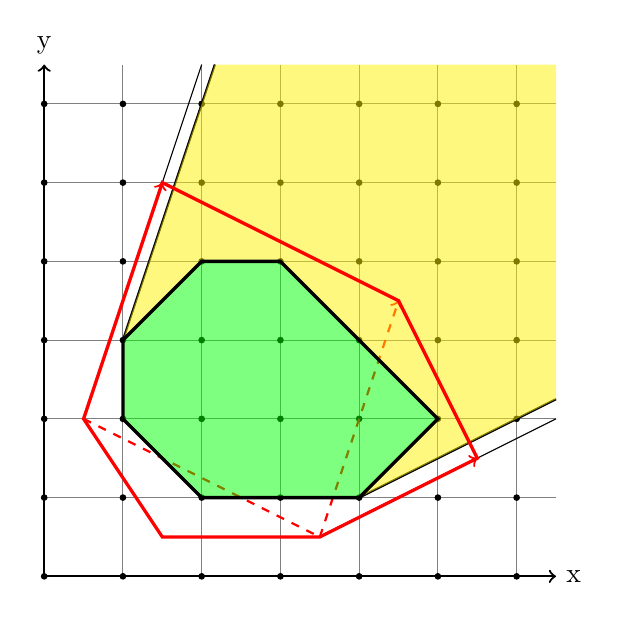
\begin{tikzpicture}
    \coordinate (extr) at (6.5, 6.5);
    \draw[style=help lines, thin] (0, 0) grid (extr);
    \draw[thick, ->] (0, 0) -- (6.5, 0) node[anchor=west] {x};
    \draw[thick, ->] (0, 0) -- (0, 6.5) node[anchor=south] {y};
    \foreach \x in {0, 1, ..., 6} {
      \foreach \y in {0, 1, ..., 6} {
        \node[draw, circle, fill=black, inner sep=0.7pt] at (\x, \y) {};
      }
    }

    \coordinate (A) at (2, 6.5);
    \coordinate (A') at (2.167, 6.5);
    \coordinate (B) at (0.5, 2);
    \coordinate (C) at (1.5, 0.5);
    \coordinate (D) at (3.5, 0.5);
    \coordinate (E) at (6.5, 2);
    \coordinate (E') at (6.5, 2.25);
    %\coordinate (B') at (6.5, 5);
    %\coordinate (D') at (5.167, 5.5);

    \coordinate (I) at (2, 4);
    \coordinate (J) at (1, 3);
    \coordinate (K) at (1, 2);
    \coordinate (L) at (2, 1);
    \coordinate (M) at (4, 1);
    \coordinate (N) at (5, 2);
    \coordinate (O) at (3, 4);

    \draw[thin] (A) -- (B);
    \draw[thin] (B) -- (C);
    \draw[thin] (C) -- (D);
    \draw[thin] (D) -- (E);

    \draw[thick] (A') -- (J);
    \draw[thick] (M) -- (E');

    \draw[red, thick, dashed, ->] (B) -- (1.5, 5);
    \draw[red, thick, dashed, ->] (D) -- (4.5, 3.5);
    \draw[red, thick, dashed, ->] (D) -- (5.5, 1.5);
    \draw[red, thick, dashed] (B) -- (D);
    \fill[fill=yellow, opacity=0.5]
      (A') -- (J) -- (I) -- (O) -- (N) -- (M) -- (E') -- (extr) -- cycle;
    \draw[very thick, fill=green, fill opacity=0.5]
      (I) -- (J) -- (K) -- (L) -- (M) -- (N) -- (O) -- cycle;
    \draw[red, very thick]
      (B) -- (C) -- (D) -- (5.5, 1.5) -- (4.5, 3.5) -- (1.5, 5) -- cycle;
  \end{tikzpicture}

  \caption{Decomposition of the integer hull of the polytope defined by the
           problem \ref{eqdecomp}}
\end{figure}

\textbf{Remark:}
Using the notations of the previous proof:
$$P \cap \ints^n \neq \emptyset \Longleftrightarrow
  P_I \neq \emptyset            \Longleftrightarrow
  (Q + B)_I \neq \emptyset      \Longleftrightarrow
  (Q + B) \cap \ints^n \neq \emptyset$$

% TODO: Cite Schriver?
Moreover, we can assume that the vectors $\{y_0, ..., y_{s-1}\}$ are linearly
independant using the fundamental theorem of linear inequalities, which implies
that $s \leqslant n$.

Finally, if $Q = \hull~\{x_0, ..., x_{k-1}\}$, then for every
$z \in Q + B$, $z \in [-B, B]^n$ where
$$B = \max_{ij} |x_{ij}| + n \cdot \max_{i, j} |y_{ij}|$$


With this remark, what remains to do is to find a bound $B$ that depends on the
parameters of the problem. To do so, a solution is to generalize the previous
theorems to bounds. % TODO: find a better formulation
We will use the notation
$\llbracket a, b \rrbracket$ for the set of integers in the interval $[a, b]$.

\begin{theorem}[Generalized Farkas-Minkowsky-Weyl Theorem]
  A set $C$ is a finitely generated cone \ifff{} is is a polyhedral cone.

  Moreover, if $C = \{x~|~Ax \leqslant 0\}$ and
  $A \in \llbracket -m, m \rrbracket^{p \times n}$ with $m \geqslant 1$,
  there exists a finite set $Y$ such that
  $Y \subseteq \llbracket -B, B \rrbracket^n$
  and $$C = \cone~Y$$ where
  $$B = (n - 1)! \cdot m^{n-1}$$
\end{theorem}

\begin{corollary}[Generalized Decomposition Theorem]
  A set of points $P$ is a polyhedron \ifff{} there exists a polytope $Q$ and a
  finitely generated cone $C$ such that $P = Q + C$.

  Moreover, if $P = \{x~|~Ax \leqslant b\}$ with
  $A \in \llbracket -m, m \rrbracket^{p \times n}$,
  $b \in \llbracket -m, m \rrbracket^p$, and $m \geqslant 1$,
  then there exists finite sets
  $Q \subseteq [-B, B]$ and $X \subseteq \llbracket -B, B \rrbracket$ such that
  $$P = \hull~Q + \cone~X$$ with $$B = n! \cdot m^n$$
\end{corollary}

We finally have the desired result:

\begin{corollary}
  If $P = \{x~|~Ax \leqslant b\}$ with
  $A \in \llbracket -m, m \rrbracket^{p \times n}$,
  $b \in \llbracket -m, m \rrbracket^p$ and $m \geqslant 1$, then
  $$P \cap \ints^n \neq \emptyset \Longleftrightarrow
  P \cap \llbracket -B, B \rrbracket^n \neq \emptyset$$ where
  $$B = (n + 1)! \cdot m^n$$
\end{corollary}

With the same ouline of proof, we can obtain a more general result that
encompasses MILPs and strict inequalities. If $I$ is a subset of
$\llbracket 1, n \rrbracket$:

\begin{theorem}
  If $P = \{x~|~Ax \leqslant b \cap A'x < b'\}$ with
  $A \in \llbracket -m, m \rrbracket^{p \times n}$,
  $b \in \llbracket -m, m \rrbracket^p$,
  $A' \in \llbracket -m, m \rrbracket^{p' \times n}$,
  $b' \in \llbracket -m, m \rrbracket^{p'}$ and $m \geqslant 1$, then

  $$\{x \in P~|~\forall x_i \in I.~x_i \in \ints\} \neq \emptyset
      \Longleftrightarrow
    \{x \in P~|~\forall x_i \in I.~x_i \in \llbracket -B, B \rrbracket\}
      \neq \emptyset$$
  where
  $$B = (n + 1)! \cdot m^n$$
\end{theorem}

\section{Formalization in Isabelle}
%TODO: Find a better introduction
As we have presented a method to solve MILPs, we can focus of their
formalization, which has been the main part of the work during this internship.
It consisted first in the formalization of Schrijvers results concerning linear
inequalities (section \ref{forlineq}), then in the implementation and the proof
of correction of a branch-and-bound algorithm (section \ref{forbb}).

%TODO: Find a better section name
\subsection{Formalization of Results concerning Linear Inequalities}
\label{forlineq}
This part concerns the formalization of the results from Schijver's book
described in section \ref{schrijverbnd}.
Also, other results including the Farkas' lemma or the Carathéodory's theorem
have been formalized.

This was done in collaboration with René Thiemann and Ralph Bottesch:
\textit{TODO: complete}
\begin{itemize}
  \item René developped results about integral and bounded vectors or matrices
    and ...
  \item Ralph focused on the demonstration of the fundamental theorem of linear
    inequalities and ...
  \item I mainly focused on the demonstration of the Farkas-Minkowsky-Weyl and
    the decomposition theorem.
\end{itemize}

In total, 5551 lines of proofs were written. The work was published in the
\textit{Archive for Formal Proofs}, a collection of proof libraries in Isabelle.
\cite{Linear_Inequalities-AFP}.

\textit{Shoud I talk about the extra work mainly done by René, such as the
preparation for the AFP submission?}

The formalization follows the outline given in section \ref{schrijverbnd}. For
example, several theorems have particular formulations including bounds:
\Snippet{farkas-minkowsky-2}
and a more general formulation:
\Snippet{farkas-minkowsky}

Where the following Isabelle notations are used:
\begin{itemize}
  \item $\mathtt{carrier\_vec}~n$ is the set of vectors $\mathbb{K}^n$
    where $\mathbb{K}$ is a field.
  \item $\mathtt{carrier\_mat}~nr~nc$ is the set of matrices
    $\mathbb{K}^{nr \times nc}$.
  \item $\mathbb{Z}_v$ is the set of integral vectors.
  \item $\mathbb{Z}_m$ is the set of integral matrices.
  \item $\mathtt{Bounded\_vec}~B$ is the set of vectors with coefficients in the
    interval $[-B, B]$.
  \item $\mathtt{Bounded\_mat}~B$ is the set of matrices with coefficients in
    the interval $[-B, B]$.
  \item $\mathtt{det\_bound}~n~m$ is $n! \cdot m^n$.
\end{itemize}

A difficulty I was confronted to is the different definitions of linear
combinations in Isabelle. Indeed, the standard definition is
$$\mathtt{lincomb}~c~V = \sum_{v \in V} c(v) \cdot v$$
where $V$ is a set of vectors and $c$ is a map from vectors to scalars.

A problem that can occur is the distributivity when we multiply this sum by
a matrix. Indeed, it is clear that
$$A \sum_i \lambda_i x_i = \sum_i \lambda_i \cdot A x_i$$. But this equality
cannotbe simply stated with the operator $\mathtt{lincomb}$. Indeed, it is
possible that there exists two vectors $x_0$ and $x_1$ such that
$A x_0 = A x_1$. If we want to express $\sum_i \lambda_i \cdot A x_i$ using
$\mathtt{lincomb}$, then the scalar coefficient associated to $A x_0$ is
neither $c(x_0)$ nor $c(x_1)$ but something like $\sum_{x . A x = A x_0} c(v)$,
which is more complicated to work with. More generally, this problem occurs
everytime we want to state the equality
$$f(\sum_i \lambda_i x_i) = \sum_i \lambda_i f(x_i)$$ where $f$ is a linear map.

To solution to tackle this problem is to use linear combinations over lists
with the following operation:
$$\mathtt{lincomb\_list}~c~V_s = \sum_{i = 0}^{i < l} c(i) \cdot v_i$$
where $V_s = [v_0, ..., v_{l-1}]$ is a list of vectors and $c$ is a function
mapping integers to scalars. 

% TODO: with the previous paragraphs, I give the impression that there are only
% advantages of using lincomb_list. It makes me confused.
This way, the distributivity of a linear map to a linear combination can be
expressed in a direct manner. To use the advantages of both definitions, we
usually define our concepts in two manners: one using sets and the other using
lists. For example, here is how non-negative linear combinations are defined,
for sets and for lists:

\Snippet{nonneg-lincomb}
\Snippet{nonneg-lincomb-list}

where $\mathtt{c}~`~\mathtt{Vs} = \{\mathtt{c}(x)~|~x \in \mathtt{Vs}\}$
is the image of the set $\mathtt{Vs}$ under $\mathtt{c}$.
We can then use this definition to define convex combinations:

\Snippet{convex-lincomb}
\Snippet{convex-lincomb-list}

and then define convex hulls:

\Snippet{convex-hull}
\Snippet{convex-hull-list}

Finally, we have to show that these two definitions are equivalent:

\Snippet{convex-hull-equivalence}
%\Snippet{finite-cone}
%\Snippet{cone}
%\Snippet{cone-list}
%\Snippet{finite-cone-iff-cone-list}
%\Snippet{farkas-minkowsky-1}

\subsection{Formalization of a Branch-and-Bound Algorithm}
\label{forbb}

The next part is the formalization of a branch-and-bound algorithm, as described
in the section \ref{bbdescr}. The idea was to state and prove the correctness of
a simple algorithm, without any optimization for the moment.

I first developped a function $\mathtt{branch\_and\_bound\_core}$ that takes
four arguments:

\section{Future Work}

\section*{Conclusion}

\bibliographystyle{plain}
\bibliography{sources}

\appendix

\section{Example: an Execution of DPLL($T$)}
\label{dpll}
Suppose that we want to solve the formula $\Phi$ given in section \ref{smt}
using DPLL($T$). First, let us interpret $\Phi$ as a SAT-formula and find an
valuation that satisfies it. For example:
\begin{itemize}
  \item Arbitrarily affects $A$ to 1. Asserts the atom $A$. Get a checkpoints
    $c_1$.
  \item To solve the clause $(\neg A \vee B)$, we must affect $B$ to 1.
    Asserts the atom $B$. Get a checkpoint $c_2$.
  \item Affects $C$ to 1. Asserts the atom $C$. Get a checkpoint $c_3$.
  \item To solve the clause $(\neg C \vee D)$, we must affect $D$ to 1.
    Asserts the atom $D$. Get a checkpoint $c_4$.
\end{itemize}

Now, we have found an valuation that satisfies $\Phi$ interpreted as a
SAT-formula. But we need to check if this valuation is compatible with an
assignment in the theory of linear arithmetic. It means that we need to find an
assignment to the conjuction $A \wedge B \wedge C \wedge D$, which is equivalent
to the system:
\begin{displaymath}
  \left\{
  \begin{array}{ccccr}
    x  & + & y & \geqslant 3 & (A) \\
    x  &   &   & \leqslant 1 & (B) \\
       &   & y & \leqslant 1 & (C) \\
    y  & - & x & < 2         & (D) \\
  \end{array}
  \right.
\end{displaymath}

But this system has no solution. The procedure $\icheck$ may retun that the
constraints $A$, $B$ and $C$ are mutually incompatible. As these three
constraints cannot be satisfied simultaneously, an assignement that satisfies
$\Phi$ must violate at least one of these constraints, so we can deduce that the
clause $(\neg A \vee \neg B \vee \neg C)$ is true. Instead of solving $\Phi$, we
will try to solve $\Phi' = \Phi \wedge (\neg A \vee \neg B \vee \neg C)$. We
need to backtrack, but we can notice that we could bactrack just before
the choice to affect $C$ to 1 was made. So let us backtrack to $c_2$, where only
$A$ and $B$ are affected.

\begin{itemize}
  \item To solve the clause $(\neg A \vee \neg B \vee \neg C)$, we must affect
    $C$ to 0. Asserts the atom $\neg C$. Get a checkpoint $c'_3$.
  \item To solve the clause $(\neg A \vee C \vee D)$, we must affect $D$ to 1.
    Asserts the atom $D$. Get a checkpoint $c'_4$.
\end{itemize}

Again, we have a valuation that satisfies $\Phi'$ interpreted as a
SAT-formula. We have to find an assignement that satisfies the conjuction
$A \wedge B \wedge \neg C \wedge D$, which is equivalent
to the system:
\begin{displaymath}
  \left\{
  \begin{array}{ccccr}
    x  & + & y & \geqslant 3 & (A) \\
    x  &   &   & \leqslant 1 & (B) \\
       &   & y & > 1         & (\neg C) \\
    y  & - & x & < 2         & (D) \\
  \end{array}
  \right.
\end{displaymath}

$\icheck$ may return the assignement $(x=1, y=2)$. Finally, the formula $\Phi$
is satisfiable, and $(x=1, y=2) \vDash \Phi$.

\section{Code of the Core of the Branch-and-Bound procedure}
\label{bbcode}

\end{document}
